\section{Study of the Italian territory}

This section is a demographic analysis of Italian situation. We want to analyse how population is distributed throughout the country to later show how this aspect affects accessibility to healthcare services.

Figure \ref{fig:pop_by_region} shows how population is distributed on a regional level, classifying each region with a graduated scale based on the total inhabitants of the region.
Five classes have been defined, assigning each class the same interval.
\footnote{Sturges's rule was applied to determine the appropriate number of bins for categorizing the data.
	It states
	\begin{equation*}
		k = \lfloor log_2 \rfloor n +1
	\end{equation*}
	where $k$ represents the number of bins to be defined and $n$ the total number of elements.\\
	To decide how many classes to define for categorizing regions: $k = \lfloor \log_2 21 \rfloor + 1 = 5$.
	Although Italy has 20 regions, the dataset counts 21 elements because Trentino-Alto Adige does not have a single NUTS-2 code. Instead, it is represented by two separate codes corresponding to its autonomous provinces.}
	
We can see from the figure that Lombardia is largely the most populated region, while Valle d'Aosta, Molise and Basilicata are the least populated.


\begin{figure}[tb]
	\centering
	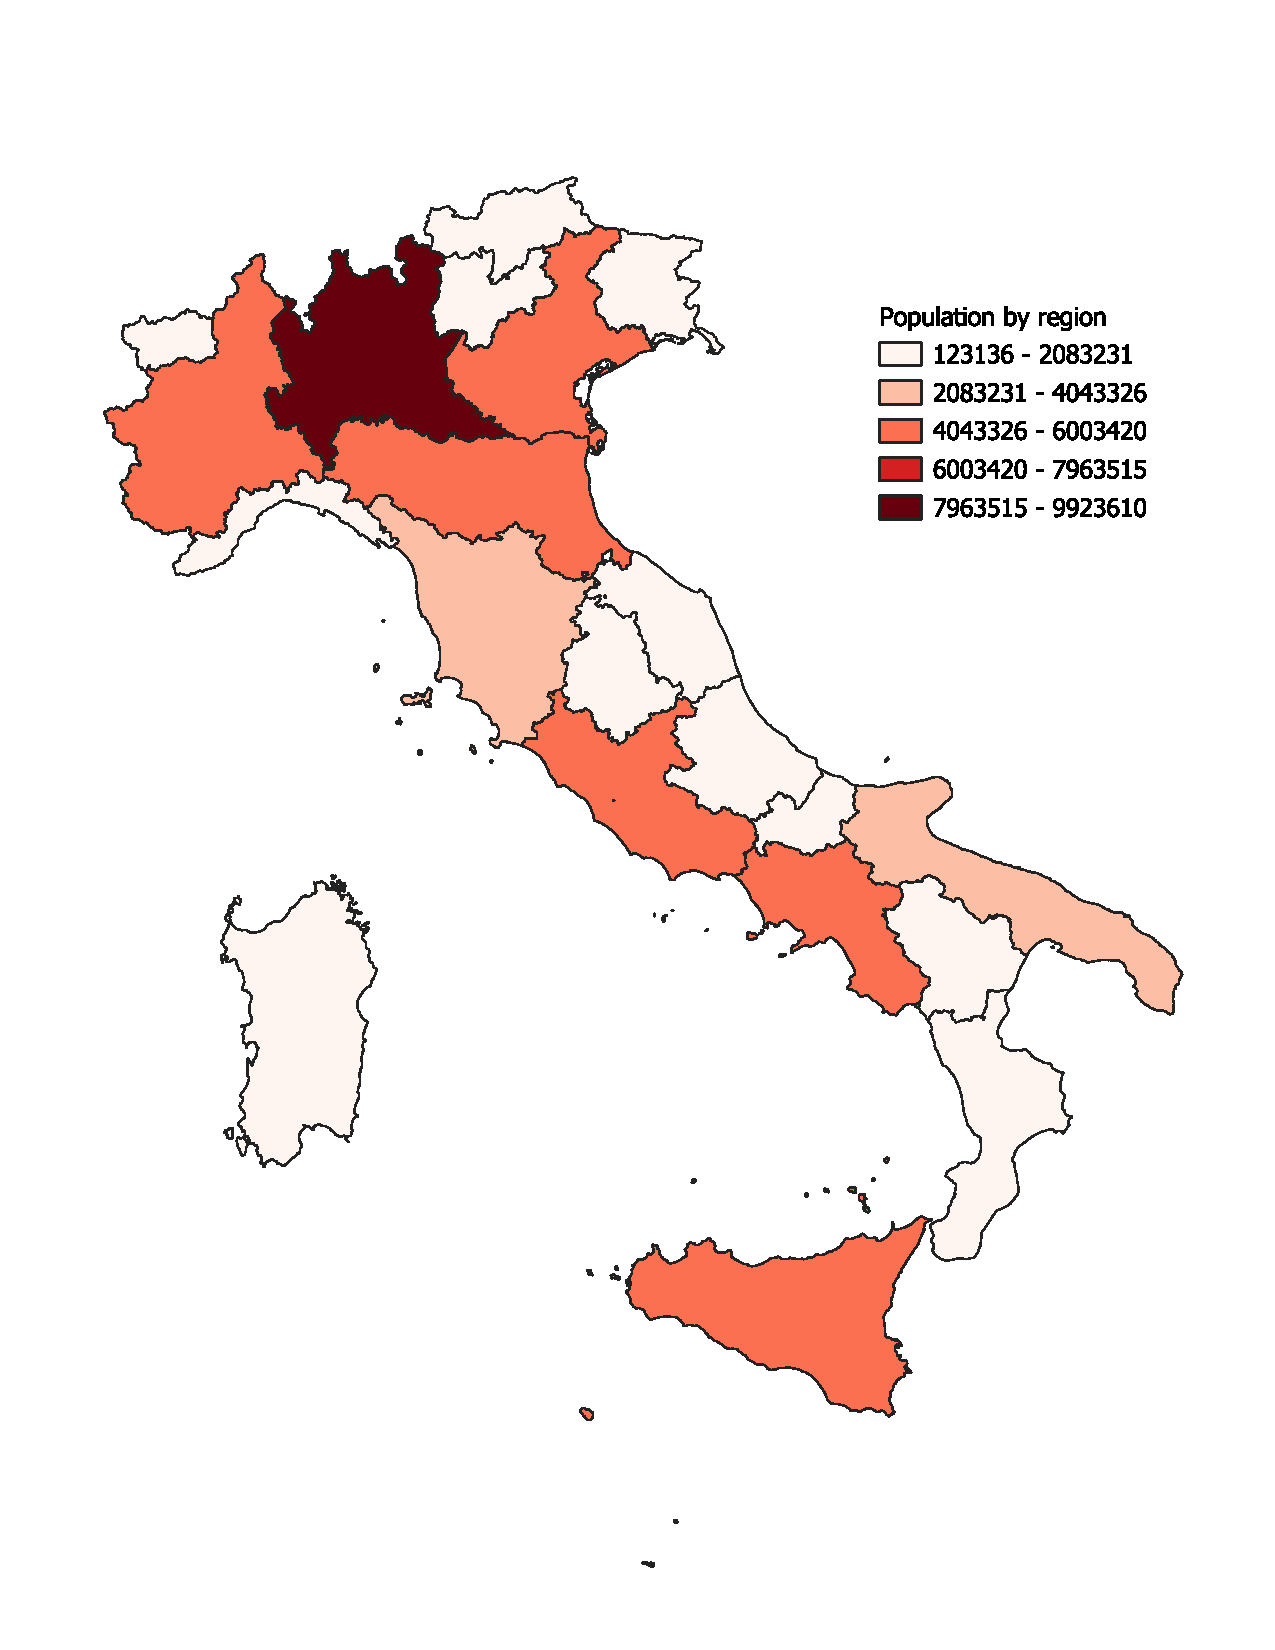
\includegraphics[width=0.8\textwidth]{img/regioni per popolazione.pdf}
	\caption{Italian population by region}
	\label{fig:pop_by_region}
\end{figure}

%\begin{figure}[tbp]
%	\centering
%	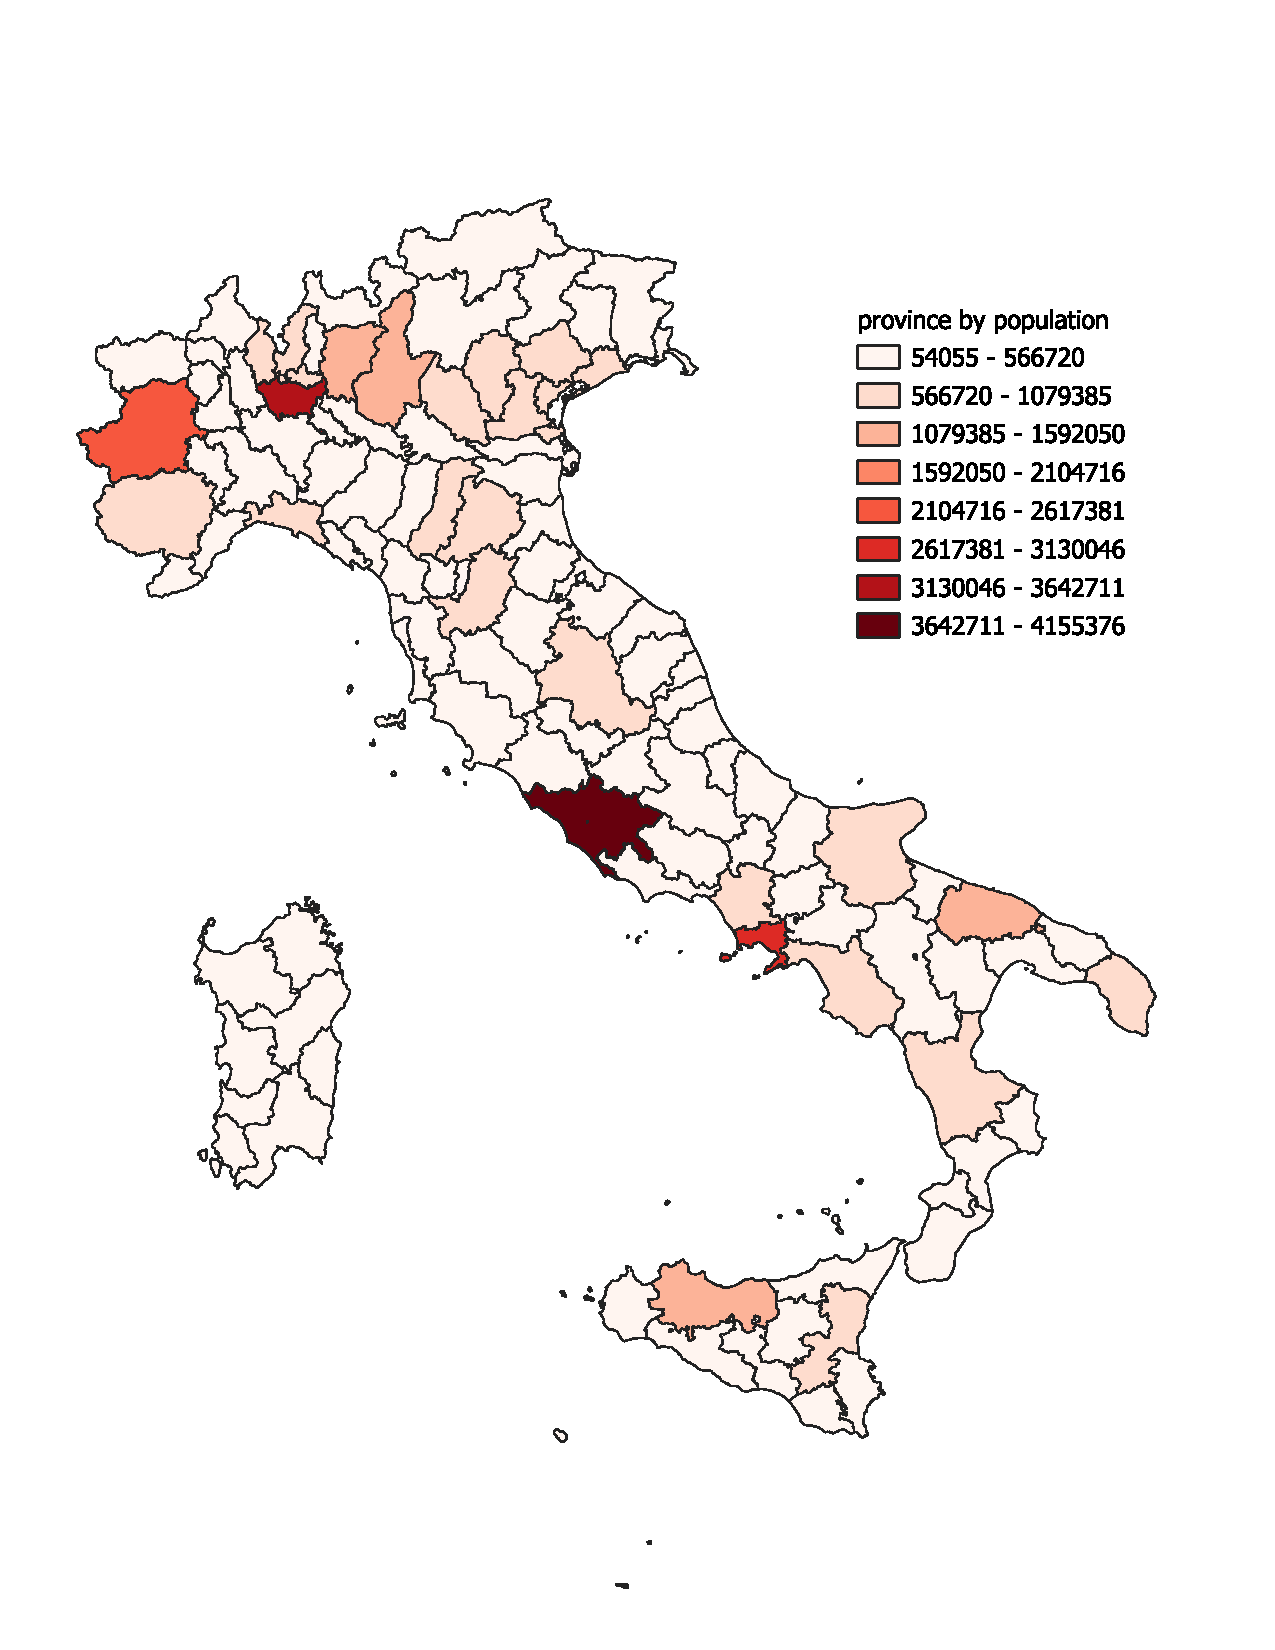
\includegraphics[width=0.8\textwidth]{img/province per popolazione.pdf}
%	\caption{Italian provinces by population}
%	\label{fig:pop_by_prov}
%\end{figure}


By increasing the resolution we can analyse how the population is distributed at the municipal level.
The graph on Figure \ref{hist:pop_by_comm} is very right-skewed, meaning that the great majority of Italian population lives in little municipalities, smaller than 50,000 inhabitants.
The graph is so right-skewed we can not even see other columns.

The chart on Figure \ref{fig:comm_by_class} illustrates the distribution of Italian municipalities by population size.
On the left axis, the blue bars represent the number of municipalities within each population class. 
The right axis shows two lines: the orange line indicates the total population (in millions) within each class, while the red dashed line shows the cumulative population across classes.

The data reveal that the vast majority of Italian municipalities are small, with populations under 10,000 inhabitants. 
However, these small municipalities account for only a limited share of the total Italian population. 
In contrast, a relatively small number of large municipalities, those with more than 100,000 inhabitants, concentrate a significant proportion of the population. 
The cumulative line clearly highlights this imbalance: only a few classes at the upper end capture the majority of residents, despite representing a minority of municipalities overall.

Table \ref{tab:comm_by_class} reports in numbers the situation described until now. 

This pattern emphasizes Italy’s demographic structure, characterized by a high number of small towns and villages, alongside a concentration of population in a limited set of large urban centres.

\begin{figure}[tbp]
	\centering
	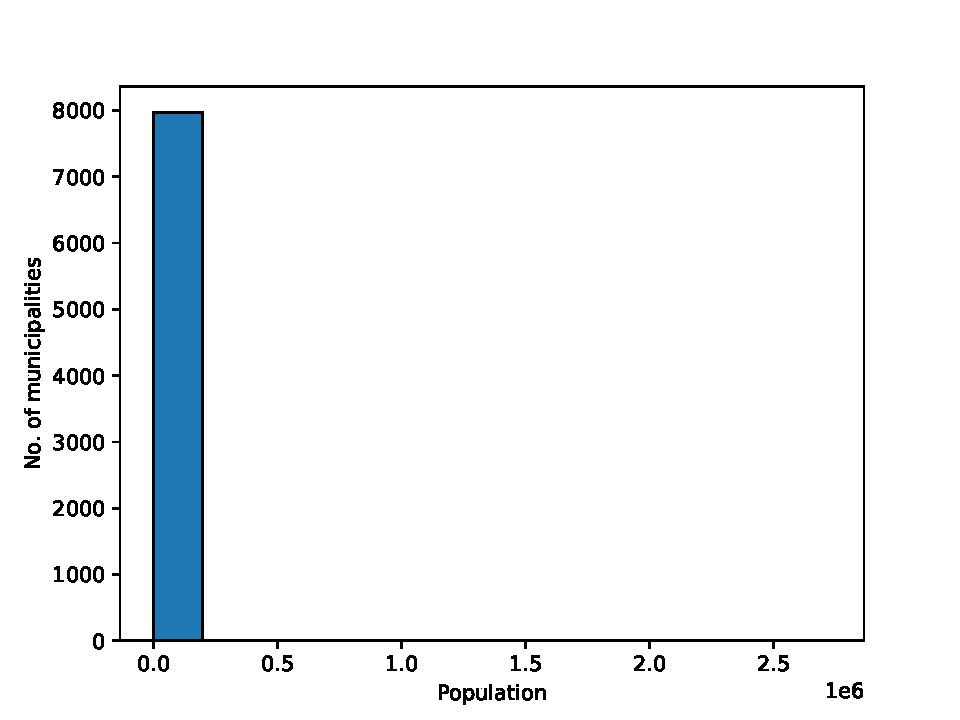
\includegraphics[width=0.8\textwidth]{img/pop_by_comm_hist.pdf}
	\caption{Distribution of population by municipality}
	\label{hist:pop_by_comm}
\end{figure}

\begin{figure}[tbp]
	\centering
	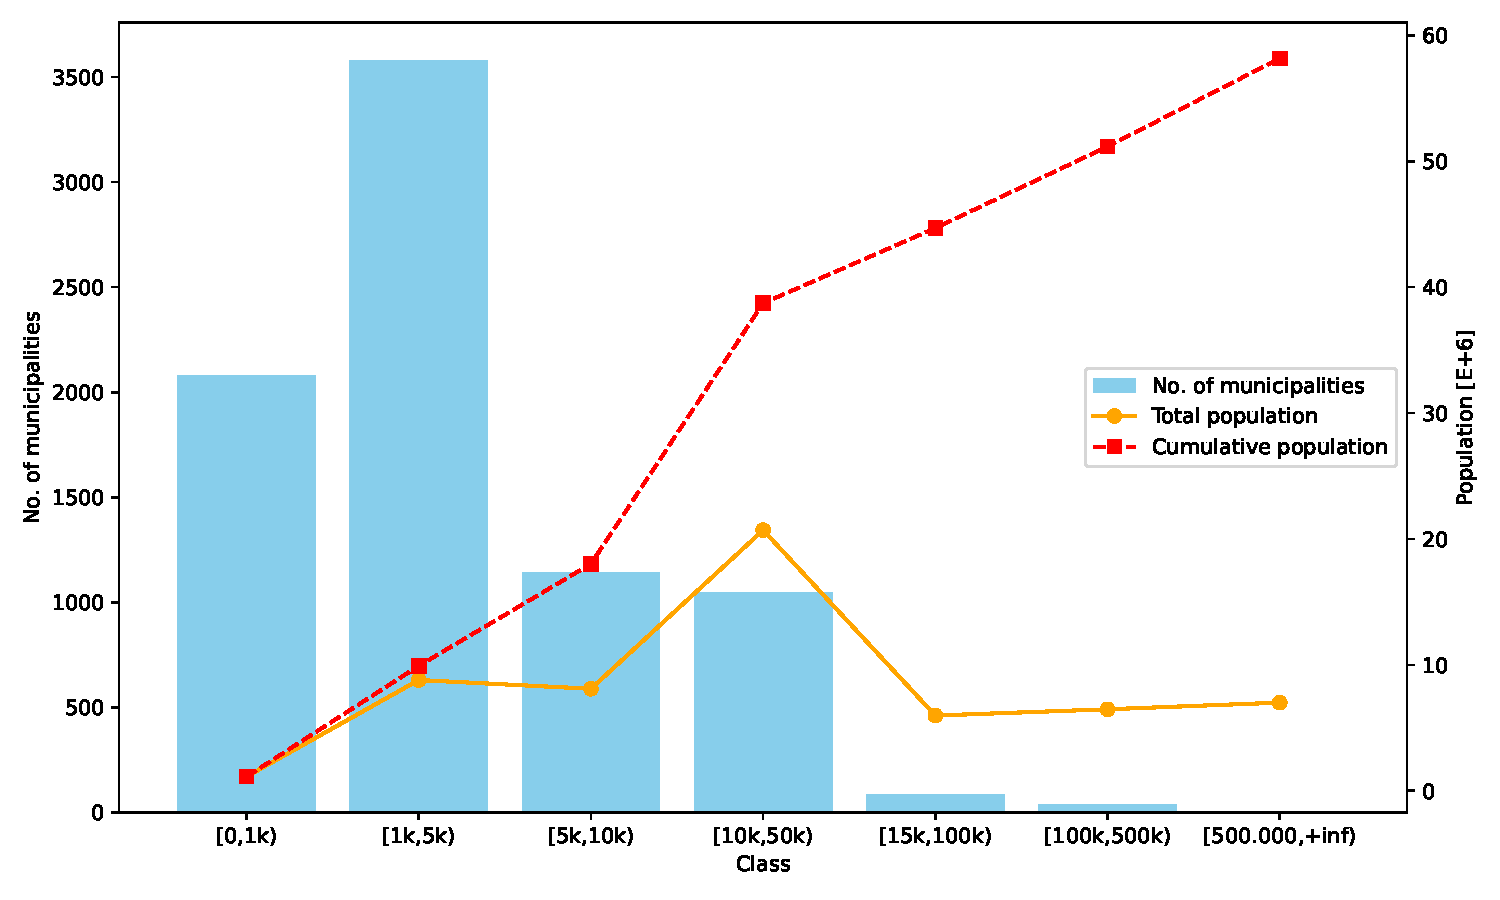
\includegraphics[width=0.8\textwidth]{img/numOfComm_by_class_v2.pdf}
	\caption{Distribution of Italian communes by population and total population living in communes of that class}
	\label{fig:comm_by_class}
\end{figure}


\begin{table}[tbp]
	\centering
\begin{tabular}{l S[table-format=4.0] S[table-format=8.0] S[table-alignment-mode = marker]}
	\toprule
	Class & \text{No. communes} & \text{Total pop.} & \text{\% on total}\\
	\midrule
	< 1.000 & 2081 & 1120526 & 1.93\\
	1.000 – 4.999 & 3580 & 8795876 & 15.12\\
	5.000 – 9.999 & 1142 & 8101451 & 13.93\\
	10.000 – 49.999 & 1048 & 20700471 & 35.59\\
	50.000 – 99.999 & 88 & 5973913 & 10.27\\
	100.000 – 499.999 & 38 & 6472224 & 11.13\\
	>= 500.000 & 6 & 7001822 & 12.04\\
	\bottomrule
\end{tabular}
	\caption{Distribution of Italian communes by population.\\
		For each category:
		number of municipalities falling within that class,
		total population residing in those municipalities,
		percentage of the national population contained in each class}
	\label{tab:comm_by_class}
\end{table}

\begin{figure}[tbp]
	\centering
	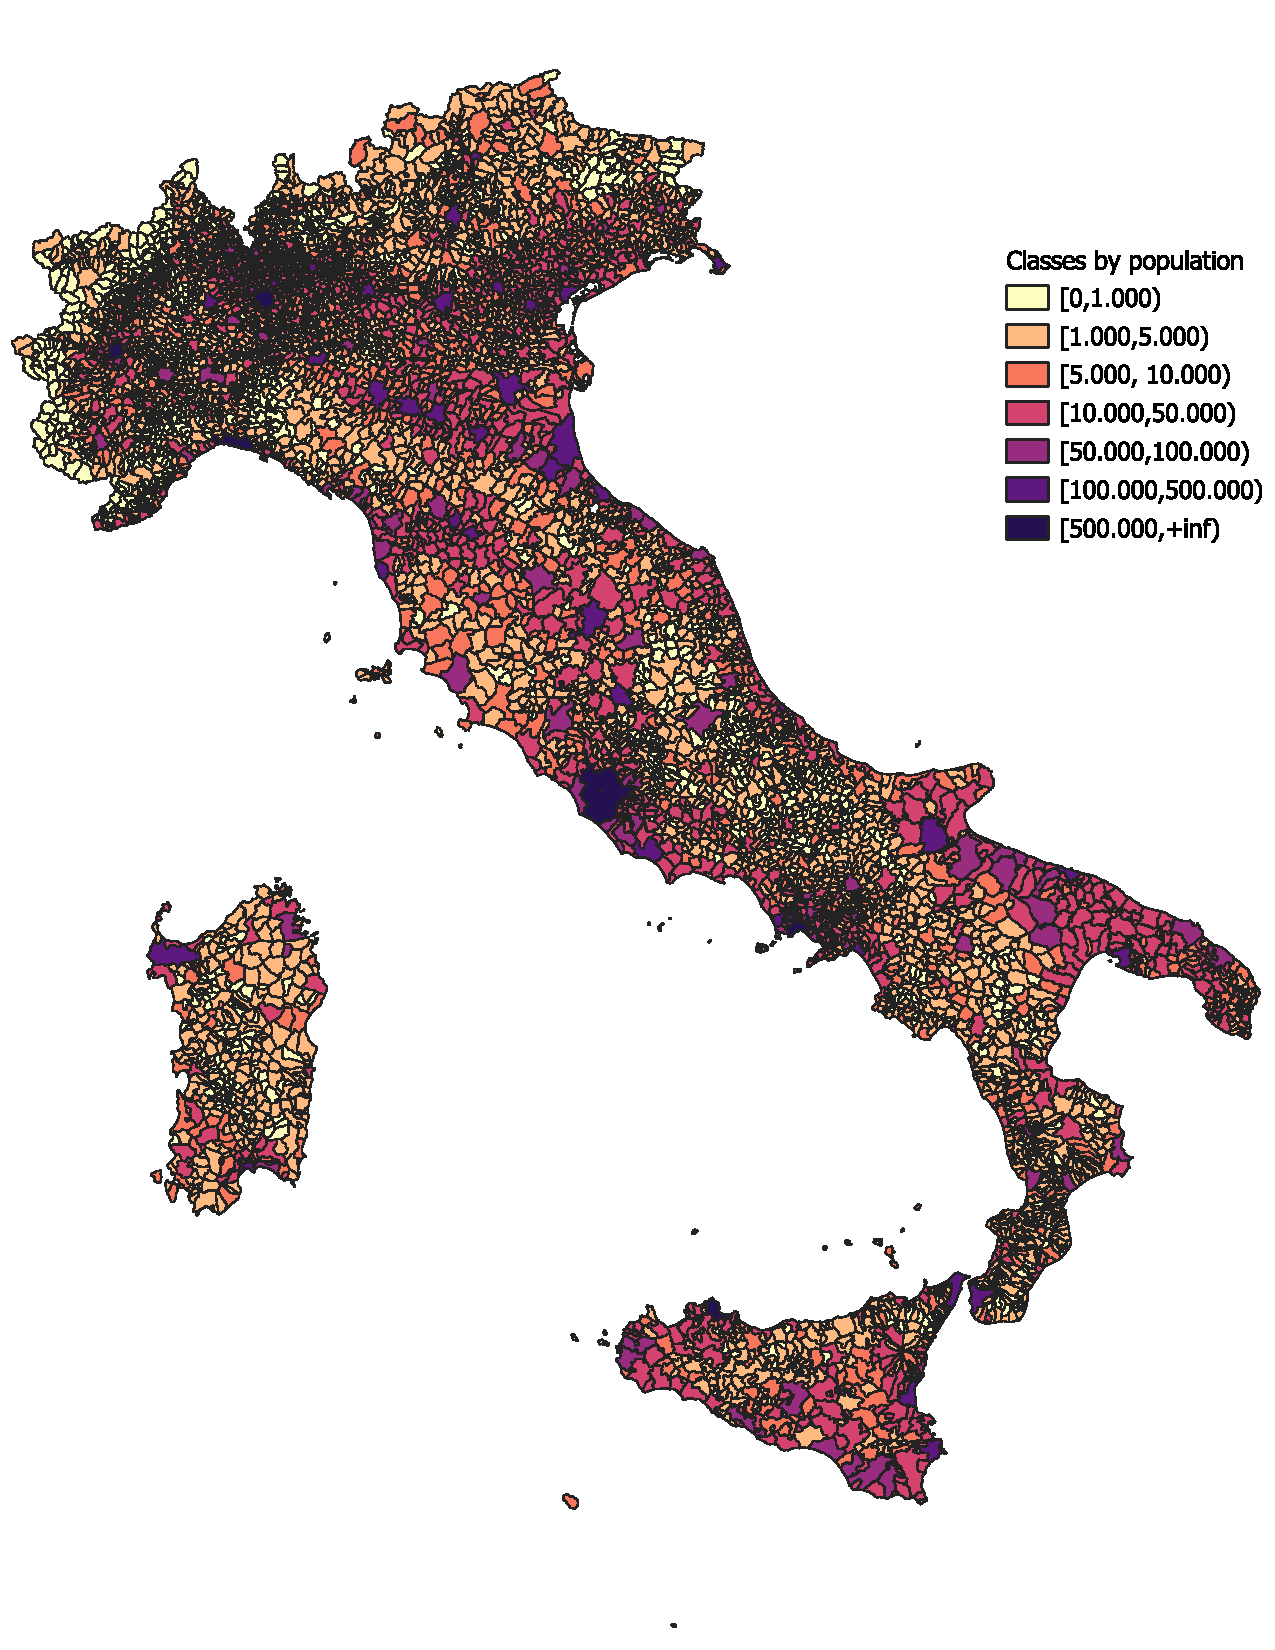
\includegraphics[width=\textwidth]{img/comuni_per_classe.pdf}
	\caption{Classification of communes by population}
	\label{map:comm_by_pop_N}
\end{figure}

% TODO possibile inserire un Treemap
% TODO inserire densità di popolazione